\documentclass{article}

\usepackage{amsmath,amssymb,amsthm,graphicx,tikz-cd,mhchem}

\usepackage{enumitem}
\usepackage{float}

\theoremstyle{definition}
\newtheorem{definition}{Definition}

% \theoremstyle{example}
% \newtheorem{example}{Example}

% \theoremstyle{remark}
% \newtheorem*{remark}{Remark}

\setlength{\oddsidemargin}{0.25 in}
\setlength{\evensidemargin}{-0.25 in}
\setlength{\topmargin}{-0.6 in}
\setlength{\textwidth}{6.5 in}
\setlength{\textheight}{8.5 in}
\setlength{\headsep}{0.75 in}
\setlength{\parindent}{0 in}
\setlength{\parskip}{0.1 in}

\newtheorem{theorem}{Theorem}
\newtheorem{corollary}{Corollary}
\newtheorem{proposition}{Proposition}
\newtheorem*{remark}{Remark}
\theoremstyle{definition}
\newtheorem{example}{Example}
\newtheorem{definition}{Definition}

\newcommand{\lecture}[4]{
   \pagestyle{myheadings}
   \thispagestyle{plain}
   \newpage
%   \setcounter{lecnum}{#1}
   \setcounter{page}{1}
   \noindent
   \begin{center}
   \framebox{
      \vbox{\vspace{2mm}
    \hbox to 6.58in { {\bf CSC~565: Graph Theory
                        \hfill North Carolina State University} }
    \hbox to 6.58in { {\bf Fall 2019
                        \hfill Computer Science} }
       \vspace{4mm}
       \hbox to 6.28in { {\Large \hfill Lecture #1: #2  \hfill} }
       \vspace{2mm}
       \hbox to 6.28in { {\it Lecturer: {\it Don Sheehy {\tt <drsheehy@ncsu.edu>}} \hfill Scribe: #4} }
      \vspace{2mm}}
   }
   \end{center}
   \markboth{Lecture #1: #2}{Lecture #1: #2}
   \vspace*{4mm}
}


\begin{document}

  \title{Lecture 2}
  \author{Scribed by: Yuhan Chen, Xianpeng Liu }
  \maketitle
  
 \section{Graph Isomorphisms} 
  \begin{definition}
  Graphs A and B are isomorphic iff $\mathbb{E}$ bijection $V_A\leftrightarrow V_B$ that maps edges to edges.
  \end{definition}
  
   \begin{figure}[h]
    \centering
      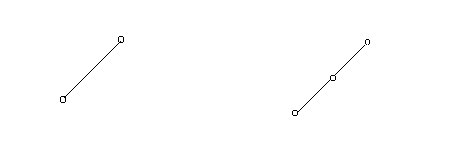
\includegraphics[width=0.6\textwidth]{fig1.png}
      \caption{Example for isomorphisms}
    \end{figure}
    
       \begin{figure}[h]
    \centering
      \includegraphics[width=0.6\textwidth]{fig2.png}
    \end{figure}
$$
\left( g\comp f \right) \left( a \right) \,\,=\,\,g\left( f\left( a \right) \right) 
$$
$$
id_A\left( a \right) \,\,=\,\,a
$$

\textbf{Inclusions} $A\cong B$ iff $
\exists f:A\rightarrow B,\,\,g:B\rightarrow A\,\,\,\,\,\,s.t.\,\,g\comp f=id_A\,\,\,\,f\comp g=id_B
$

\section{The Category Set}

  \begin{theorem}
    The set $\mathbb{Z}_+$ of positive integers is not isomorphic to the set X of sets of positive integers.
  \end{theorem}
  \begin{proof}
    Suppose the set $\mathbb{Z}_+$ of positive integers is isomorphic to the set X of sets of positive integers. which means 
  \begin{tikzcd}
\mathbb{Z}_+ \arrow[shift left=2pt]{r}{f} & X\arrow[shift left=2pt]{l}{g}
\end{tikzcd}, $f\comp g=id_X,\,\,\,\,g\comp f=id_{\mathbb{Z}_+}$,
Let 
$$S=\left\{ i\in \mathbb{Z}_+:\,\,i\notin f\left( i \right) \right\} $$
$$S=id_X\left( S \right) =\left( f\comp g \right) \left( S \right) =f\left( g\left( S \right) \right) $$
Is $g(S)\in S$, let $i=g(S)$. Then we can get $g(S)\in S$ iff $g(S)\notin S$, which is impossible.
   \begin{figure}[h]
    \centering
      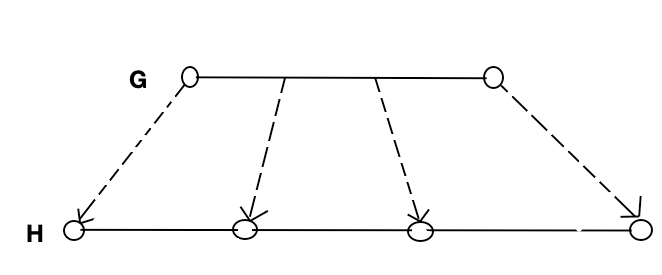
\includegraphics[width=0.5\textwidth]{fig3.png}
      \caption{Example for set S}
    \end{figure}
  \end{proof}

\section{Graph Morphisms}

\begin{definition}
A morphism is $G\rightarrow H$ is a function $f:V_G\rightarrow V_H$ 
$$s.t.\forall\left( u,v \right)\in E_G$$ 
we have $\left( f\left( u \right) ,f\left( v \right) \right) \in E_H$
\end{definition}

\newpage 

\section{Some Special Graphs}

\quad \textbf{(1)}. \underline{Clique} or \underline{Complete Graph} on n vertices $K_n$
   \begin{figure}[h]
    \centering
      \includegraphics[width=0.6\textwidth]{fig4.png}
    \end{figure}
    
\textbf{(2)}. \underline{Path} $P_m$ with m edges, "length of $P_m$" is the number of edges (m)
   \begin{figure}[h]
    \centering
      \includegraphics[width=0.7\textwidth]{fig5.png}
    \end{figure}
    
\textbf{(3).} \underline{Cycle}
   \begin{figure}[h]
    \centering
      \includegraphics[width=0.7\textwidth]{fig6.png}
    \end{figure}
    
\textbf{(4).} \underline{Bipartite Graphs}, $G=\left( A\cup B,E \right) $, where $E \in A \times B$ and $S \cap B = \oslash $
   \begin{figure}[h]
    \centering
      \includegraphics[width=0.3\textwidth]{fig7.png}
    \end{figure}
    
\newpage
\textbf{(5).} \underline{Complete Bipartite Graphs}, $K_K_{a,b}$. All edges from every vertex of A to every vertex of B. $$K_{a,b}=\left( \left[ a \right] \sqcup \left[ b \right] ,\left[ a \right] \times \left[ b \right] \right)$$
\begin{figure}[h]
\centering
  \includegraphics[width=0.8\textwidth]{fig8.png}
\end{figure}

\underline{Claim}:Graph with at least two vertices is bipartite iff you can map it's morphism to a graph into $K_2$

\section{Subgraphs}
\begin{definition}
    $G=(V,E)$, $G' =\left( V' ,E'  \right)$, G is subgraph of G'($G\subseteq G'$) iff $V\subseteq V'$ and $E\subseteq E'$
\end{definition}

\underline{Edits}
$$
G+e\,\,or\,\,G\cup e\,\,=\,\,\left( V,\,\,E\cup e \right) 
$$$$
G+v\,\,or\,\,G\cup v\,\,=\,\,\left( V\cup v,\,\,E \right) 
$$$$
G\setminus v\,\,or\,\,G-v\,\,=\,\,\left( V\setminus \left\{ v \right\} ,\,\,E\setminus \left( \left\{ v \right\} \times V \right) \right) 
$$

\section{Induced Subgraphs}
\begin{definition}
    $G=(V,E)$, G' is an induced subgraph (on V') iff $G'=(V', E\cap (V'\times V')$, $V'\subsetqu V$, $G'=G\setminus \left( V\setminus V' \right) $
\end{definition}
    
\end{document}
